\documentclass[10pt]{exam}
\usepackage[utf8]{inputenc}		% Caracteres latinos
\usepackage[spanish]{babel}		% Idioma español
\usepackage{geometry}			% Organizar el documento
\usepackage{graphicx}			% Incluir gráficos
\usepackage{makecell}			% Para personalizar las celdas de una tabla
\usepackage[nohdr]{mathexam}	% Añadimos el paquete mathexam (sin header)
\usepackage{amsmath}
\usepackage{amsfonts}
\usepackage{amssymb}
\usepackage{mathtools}
\usepackage{tikz,pgfplots}
\usepgfplotslibrary{polar}
\usepackage[shortlabels]{enumitem}
 \renewcommand{\baselinestretch}{1.5}

%\usepackage[]{mathptmx}        % A free version o Times Roman with mathematical symbols
%\usepackage{pzc}               % fuente cursiva (conjuntos) Zapf Chancery
%\usepackage{showframe}
%\usepackage{lipsum}

% DOCUMENTACIÓN DE LA CLASE EXAM
% http://ftp.inf.utfsm.cl/pub/tex-archive/macros/latex/contrib/exam/examdoc.pdf
% DOCUMENTACIÓN DE LA CLASE MATHEXAM
% http://ctan.dcc.uchile.cl/macros/latex/contrib/mathexam/doc/mathexam.pdf

% Definimos la geometría de la primera página
\geometry{
	a4paper,                    % Tamaño del documento
	hmargin = {1.5cm, 1.5cm}, 	% Margen horizontal izquierdo, derecho
	vmargin = {0.5cm, 1cm},	    % Margen vertical superior, inferior
	headsep = 4mm,				% Separación entre el encabezado y el texto
	head = .2cm,				% Tamaño del encabezado
	% marginparsep = 5mm, 		% Seperación entre las notas y el texto
	% marginpar = 1.5cm,		% Tamaño de las notas
	includeall,                 % incluye el encabezado, footer y notas dentro del tamaño del documento
	nomarginpar,	            % Elimina las notas
	foot = 1cm,                 % Tamaño del footer
	twoside,                	% Habilita el modo de impresión a doble cara
}

\selectlanguage{spanish}        % Selecciona el idioma
\spanishdecimal{.}

%\pagestyle{headandfoot}         % Nuestro examen tendrá encabezado y pié

% DEFINIMOS EL ENCABEZADO
%\header{
%\begin{tabular}{l c c c l}
%            \makecell{\includegraphics[height=2.5cm]{logo.png}} &
%            \makecell{\textbf{IPEA 215} \\Raúl Scalabrini Ortiz} &
%            \makecell{Examen} &
%            \makecell{Curso\\1er Año} &
%             \makecell[l]{Apellido y %Nombre:\enspace\makebox[2in]{\hrulefill}\\Fecha: \today}
%        \end{tabular}}{}{}

% DEFINIMOS EL PIE
%\rfoot{Página \thepage\ de \numpages}

% DOCUMENTO
\begin{document}

\centering


\Large 
\textbf{Tarea 2}

\normalsize
Fecha de entrega: 

Miércoles 04/09/2024 durante la clase




\pointpoints{punto}{puntos}
\pointformat{\bfseries\boldmath(\thepoints)}
\vskip10pt

\begin{questions}
    \question 
    
    \begin{enumerate}[a)]
        \item Obtén la ecuación de la parábola con vértice en el origen, su eje sobre el eje $y$ y que pasa por el punto $(-2,4)$. Dibuja la parábola.
        \item Uno de los cables de un puente colgante pende en forma de parábola cuando la carga está uniformemente distribuida de manera horizontal. La distancia entre las dos torres es de 150 m, los puntos de soporte del cable están 22 m arriba de la carretera, y el punto más bajo del cable está 7 m sobre dicha carretera. Determina la distancia vertical de la carretera al cable de un punto que se encuentra a 15 m de la base de una torre.
    \end{enumerate}{}

    \question 
    \begin{enumerate}[a)]
        \item Dada la ecuación de la elipse $4x^2+y^2+8x-4y-92=0$, determina el centro, el eje principal, los vértices, los extremos del eje menor y los focos. Dibuja la elipse y muestra los focos.
        \item La órbita de la Tierra alrededor del Sol es de forma elíptica, con el Sol en uno de sus focos y un semieje mayor de longitud de 92.96 millones de millas. Si $c/a=0.0167$, determina las distancias mínima (perihelio) y máxima (afelio) entre la Tierra y el Sol.
    \end{enumerate}{}
    
    \question 
    \begin{enumerate}[a)]
        \item Considera la ecuación de la hipérbola $\frac{x^2}{4}-\frac{y^2}{4}=1$. Obtén el centro, el eje principal y los vértices. Dibuja la hipérbola y las asíntotas.
       % \item Obtén la ecuación de la hipérbola con centro en el origen, los focos sobre el eje $y$ y que pasa por los puntos $(-2,4)$ y $(-6,7)$.
        \item En el sistema de navegación por radio LORAN (LOng RAnge Navigation), dos estaciones de radio localizadas en $A$ y $B$, transmiten en forma simultánea señales a un barco o avión localizado en $P$. La computadora de a bordo convierte la diferencia de tiempo de recibir estas señales en una diferencia de distancia , y esto, de acuerdo con la definición de una hipérbola, localiza al barco o avión en una rama de una hipérbola. Suponga que la estación $B$ se localiza a 400 millas al este de la estación $A$ sobre la costa. Un barco recibe la señal de B 1200 microsegundos ($\mu$s) antes de recibir la señal de $A$.
        \begin{enumerate}[i)]
        \item Si se supone que la señal de radio viaja a una rapidez de 980 pies/$\mu$s, encuentra la ecuación de la hipérbola sobre la que se localiza el barco.
        \item Si el barco se dirige al norte de $B$, ¿qué tan lejos de la costa está el barco?
         \end{enumerate}{}

        \centering
      \vskip15pt
 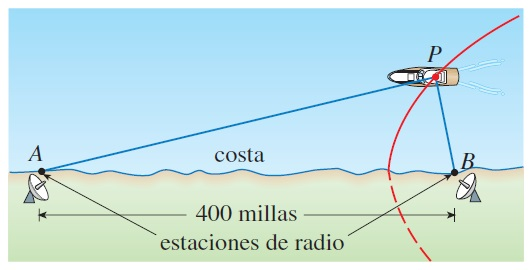
\includegraphics[scale=1]{Hiperbola.jpg}

    \end{enumerate}{}

   \question
   En cada función determina donde se puede invertir la función, encuentra la función inversa y dibuja ambas funciones. 
   \begin{enumerate}[a)]
   \item $f(x)=(x-2)^3$
   \item $f(x)=\dfrac{x}{1-x^2}$
   \end{enumerate}

    
    \end{questions}


% Geometría para la otra carilla
\newgeometry{
	hmargin = {1.5cm, 0.5cm},
	vmargin = {0.5cm, 1cm},
	%nofoot,			% Elimina el pié
	nohead,			% Elimina el encabezado
	nomarginpar,	% Elimina las notas
	includeall,
}% \savegeometry{geometria_1}

\pagestyle{foot}    % El estilo de ésta página sólo constará de pié de página
\runningfooter{}{}{Página \thepage\ de \numpages}


%\lipsum[1-5]

% \restoregeometry
% \loadgeometry{geometria_1}


\end{document}